\documentclass[tikz,border=4pt]{standalone}
\usepackage{amsmath}
\begin{document}
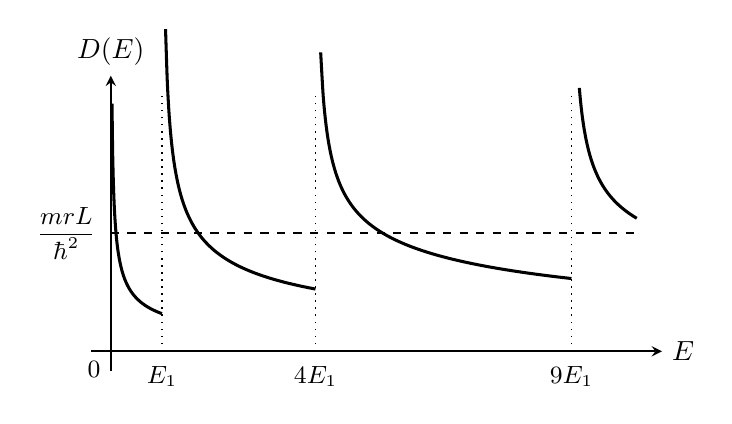
\begin{tikzpicture}[>=stealth, thick, scale=1.0]
  % Axes: x = E / (E_1 * 2.5) so E_1 = 0.65, 4 E_1 = 2.60, 9 E_1 = 5.85
  % Let x_1 = 0.65 (l=1), x_2 = 2.60 (l=2), x_3 = 5.85 (l=3)
  \draw[->, line width=0.65pt] (-0.25, 0) -- (7.0, 0) node[right] {$E$};
  \draw[->, line width=0.65pt] (0, -0.25) -- (0, 3.5) node[above] {$D(E)$};
  \node[below left, font=\small] at (0, 0) {$0$};

  % 2D average asymptote D_2D = m r L / hbar^2 -> scaled to y = 1.5
  % Check exact scaling: D_cyl(E) / D_2D = (1/pi) * [1/sqrt(u) + 2 sum_{l>=1} 1/sqrt(u - l^2)] where u = E/E_1 = x / 0.65
  % So y(x) = (1.5 / pi) * [1/sqrt(u) + 2 sum 1/sqrt(u - l^2)]
  \draw[dashed, line width=0.7pt] (0, 1.5) -- (6.7, 1.5);
  \node[left, font=\small] at (-0.06, 1.5) {$\dfrac{mrL}{\hbar^2}$};

  % Vertical asymptotes at E_1, 4 E_1, 9 E_1
  \draw[dotted, line width=0.55pt] (0.65, 0) -- (0.65, 3.25);
  \draw[dotted, line width=0.55pt] (2.60, 0) -- (2.60, 3.25);
  \draw[dotted, line width=0.55pt] (5.85, 0) -- (5.85, 3.25);

  % Segment 0 < x < 0.65 (l = 0 only)
  \draw[line width=1.1pt, domain=0.015:0.65, samples=80, smooth]
    plot (\x, {0.4775 / sqrt(\x/0.65)});

  % Segment 0.65 < x < 2.60 (l = 0, +-1)
  \draw[line width=1.1pt, domain=0.695:2.60, samples=90, smooth]
    plot (\x, {0.4775 * (1/sqrt(\x/0.65) + 2/sqrt(\x/0.65 - 1))});

  % Segment 2.60 < x < 5.85 (l = 0, +-1, +-2)
  \draw[line width=1.1pt, domain=2.665:5.85, samples=100, smooth]
    plot (\x, {0.4775 * (1/sqrt(\x/0.65) + 2/sqrt(\x/0.65 - 1) + 2/sqrt(\x/0.65 - 4))});

  % Segment 5.85 < x < 6.7 (l = 0, +-1, +-2, +-3)
  \draw[line width=1.1pt, domain=5.95:6.68, samples=60, smooth]
    plot (\x, {0.4775 * (1/sqrt(\x/0.65) + 2/sqrt(\x/0.65 - 1) + 2/sqrt(\x/0.65 - 4) + 2/sqrt(\x/0.65 - 9))});

  % Ticks on E-axis
  \node[below, font=\small] at (0.65, -0.06) {$E_1$};
  \node[below, font=\small] at (2.60, -0.06) {$4E_1$};
  \node[below, font=\small] at (5.85, -0.06) {$9E_1$};
\end{tikzpicture}
\end{document}
